\documentclass[12pt]{article}
\usepackage[utf8]{inputenc}
\usepackage{polski}
\usepackage[a4paper, left=2.0cm, right=2.0cm, top=2.0cm, bottom=2.0cm]{geometry}
\usepackage{graphicx}
\usepackage{multicol}


\title{PIISW, W08, IO, 2020/2021, semestr letni\\Lista zadań nr 2: HTML, CSS i~Javascript}
\author{mgr inż. Maciej Małecki\\\small{maciej.malecki@pwr.edu.pl}}

\begin{document}
    \maketitle

    \section*{Wprowadzenie}
    \begin{itemize}
        \item Rozwiązania zadań z~tej listy muszą znaleźć się w~nowym prywatnym repozytorium na \texttt{github.com}.
        \item Prowadzący zajęcia musi mieć uprawnienia do odczytu i~zapisu do tego repozytorium.
        \item Rozwiązanie każdego zadania musi się znaleźć w~podkatalogu \texttt{zadanie\_x}, gdzie \texttt{x} jest numerem zadania.
		\item Do uruchomienia skryptów napisanych w~ramach listy najlepiej użyć środowiska NodeJS.
        \item Do wykonania zadań z~zakresu HTML/CSS należy użyć dowolnej przeglądarki internetowej (tworzymy pliki źródłowe \texttt{*.html} oraz \texttt{*.css}).
    \end{itemize}

    \section*{Oceny}
    \begin{tabular}{|l|c|c|c|c|c|c|}
        \hline
        Punkty: & $<7$ & $7-8$ & $9-10$ & $11-12$ & $13-14$ & 15\\
        \hline
        Ocena:  & $2,0$ & $3,0$ & $3,5$ & $4,0$ & $4,5$ & $5,0$\\
        \hline
    \end{tabular}

    \section*{Zadania}
    \begin{enumerate}
        \item\label{exc:html-css}
            (3 pkt) Dane są dokument HTML:
            \begin{verbatim}
<!doctype html>
<html>
    <head>
      <link rel="stylesheet" href="zad1.css" type="text/css"/>
    </head>
    <body>
        <ul>
          <li>1</li><li>2</li><li>3</li><li>4</li>
          <li>5</li><li>6</li><li>7</li><li>8</li>
          <li>9</li><li>10</li><li>11</li><li>12</li>
        </ul>
        <p>Sample description</p>
    </body>
</html>
            \end{verbatim}
            oraz arkusz stylów CSS:
            \begin{verbatim}
ul:after {
  display:block;
  height:0;
  content:'';
  clear:both;
}
            \end{verbatim}
            Modyfikując jedynie arkusz styli CSS spraw, aby dokument HTML został wyrenderowany przez przeglądarkę w~sposób pokazany na rysunku~\ref{fig:css-float}.
            \begin{figure}[hb]
                \centering
                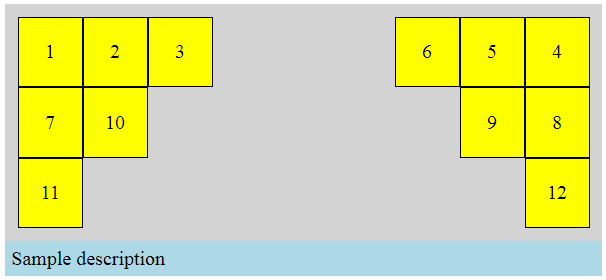
\includegraphics{css-float}
                \caption{Prawidłowo wystylowany przykład dla zadania~\ref{exc:html-css}}.
                \label{fig:css-float}
            \end{figure}

            \textbf{Wskazówki:} Zapoznaj się z~selektorem \texttt{nth-child(x)}.
        \item\label{exc:javascript-classic}
            (3 pkt) Napisz program w~języku Javascript, który akceptuje dowolną ilość liczb całkowitych jako argumentów wejściowych oraz wyświetla numeryczny wynik na wyjściu będący sumą: argumentów powiększonych o $1$, jeśli argumenty są liczbami nieparzystymi oraz argumentów pomniejszonych o $1$, jeśli argumenty są liczbami parzystymi.

            Program należy napisać ,,klasycznie'', z~wykorzystaniem pętli \texttt{for} oraz instrukcji warunkowej.

            Przykładowe wyniki działania programu:
            \begin{multicols}{2}
                \begin{itemize}
                    \item $\emptyset\rightarrow$ \texttt{0}
                    \item \texttt{0} $\rightarrow$ \texttt{-1}
                    \item \texttt{1} $\rightarrow$ \texttt{2}
                    \item \texttt{1 2 3} $\rightarrow$ \texttt{7}
                \end{itemize}
            \end{multicols}
        \item
            (5 pkt) Przepisz program z~zadania~\ref{exc:javascript-classic} z~wykorzystaniem technik programowania funkcyjnego tak, aby wyeliminować konieczność użycia instrukcji: pętli, warunkowych oraz deklaracji zmiennych.

            \textbf{Wskazówka:} użyj funkcji \texttt{filter}, \texttt{map}, \texttt{reduce}.
        \item
            (4 pkt) Rozwiń następujący przykład z~wykładu:
            \begin{verbatim}
var account = {
  balance: 0,
  debit: function(amount) {
    if (amount < 0) { throw new Error('Illegal amount'); }
    if (this.balance < amount) {
        throw new Error('Insufficient account balance');
    }
    this.balance -= amount;
    return this.balance;
  },
  credit: function(amount) {
    if (amount < 0) {
        throw new Error('Illegal amount');
    }
    this.balance += amount;
    return this.balance;
  }
};
            \end{verbatim}
            tak, aby
            \begin{enumerate}
                \item umożliwić tworzenie wielu obiektów o~identycznej strukturze jak obiekt \texttt{account},
                \item rozszerzyć listę pól obiektu o~następujące pola: numer konta, data utworzenia, waluta,
                \item uniemożliwić bezpośrednią manipulację wartością atrybutów \texttt{balance}, nr konta, data utworzenia oraz waluta,
                \item umożliwić inicjalizację wszystkich pól poza \texttt{balance} dowolnie wybranymi wartościami w~momencie tworzenia obiektu (później wartości tych atrybutów powinny być niezmienne),
                \item umożliwić odczyt wartości wszystkich atrybutów przy pomocy pojedynczego wywołania metody oraz obiektu opisującego.
            \end{enumerate}
            \textbf{Wskazówka}: użyj metody fabrykującej oraz techniki domknięcia (\emph{closure}).
    \end{enumerate}
\end{document}

